% -----------------------------*- LaTeX -*------------------------------
\documentclass[11pt]{report}
\usepackage{scribe_ds603}
\begin{document}


\scribe{Ritik}		% required
\lecturenumber{6}			% required, must be a number
\lecturedate{22/08/2025}		% required, omit year

\maketitle

% ----------------------------------------------------------------------


\section{Revisitng supervised learning}
\subsection{Training vs. Testing}
During \textbf{training/estimation}: We have data points
\[
    z_i = (x_i, y_i) \sim \mathbb{P^*}, \quad i = 1, \dots, n
\] 
where $\mathbb{P^*}$ is the true data distribution. Using this training set, we contruct the \textbf{empirical distribution} which is defined as
\[
    \hat{\mathbb{P}}_n = \frac{1}{n} \sum_{i=1}^n \delta_{z_i}.
\]
Here, $\delta_{z_i}$, is the \textbf{Dirac measure}~\cite{lax2014functional} at the point $z_i$ (a probability mass concentrated at that sample).
\\
\\
During \textbf{testing/inference}: Samples $z=(x,y)$ are assumed to be drawn from the true distribution $\mathbb{P^*}$.

\subsection{Dirac Measure}
For a measurable space $(X, \mathcal{F})$, the Dirac measure at a point $x \in X$ is defined as
\[
    \delta_x(A) = \mathbf{1}_A(x) = 
    \begin{cases}
        1 & \text{if } x \in A, \\
        0 & \text{if } x \notin A,
    \end{cases}
    \quad \forall A \in \mathcal{F}.
\]
\underline{\textbf{Note:}} The Dirac measure is a \textbf{probability measure}. For any measurable function $f$,
\[
    \int_{x} f(y)\, d\delta_x(y) = f(x).
\]
See Appendix~\ref{adx1} for proof.\\ \\
\textbf{Question:} Is $\hat{\mathbb{P}}_n$ a discrete measure.

Yes it is a discrete measure, because it is a finite sum of weighted Dirac measuresa. A general discrete measure can be expressed as
\[
    \mu = \sum_{i} a_i \, \delta_{x_i}, \quad a_i \geq 0.
\]

The empirical distribution $\hat{\mathbb{P}}_n$ is a discrete measure with uniform weights $a_i = \tfrac{1}{n} \text{ and also note} \sum_{i} a_i = 1$.

\subsection{Learning via Optimization}
The \textbf{true risk minimization} problem is
\[
    \min_{\theta \in \Theta} \, \mathbb{E}_{z \sim \mathbb{P^*}} \big[ \ell(\theta, z) \big] 
    = \min_{\theta} \int_z \ell(\theta, z) \, d\mathbb{P^*}(z).
\]
That is \textbf{expected loss} under the true distribution $\mathbb{P^*}$.
Since $\mathbb{P^*}$ is unknown, we approximate using the \textbf{empirical risk}:
\[
    \min_{\theta \in \Theta} \, \mathbb{E}_{z \sim \hat{\mathbb{P}}_n} \big[ \ell(\theta, z) \big] 
    = \frac{1}{n} \sum_{i=1}^n \ell(\theta, z_i).
\]

This is the principle of \textbf{Empirical Risk Minimization (ERM)}~\cite{uml}.

\subsection{Parameter Estimation}
The goal is to learn $\hat{\theta} : \mathcal{P}(z) \to \Theta$ such that
\[
    \mathbb{E}_{z \sim \mathbb{P^*}} \big[ \ell(\hat{\theta}(\hat{\mathbb{P}}_n), z) \big]
\]
is minimized.

\subsubsection{Example (Squared Loss)}
Using squared loss 
\[
    \ell(\theta, z) = \|\theta - z\|^2,
\]
the optimal $\theta$ corresponds to the \textbf{mean} of the distribution. 

\section{Data-Driven Decision Making Cycle}
\begin{figure}[h]
    \centering
    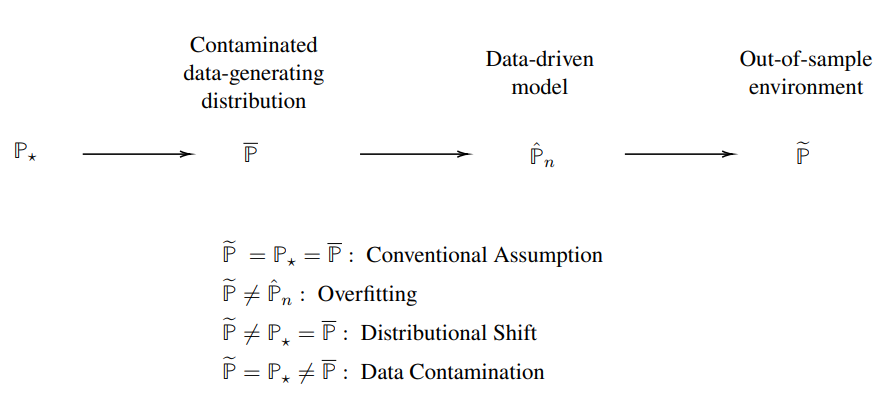
\includegraphics[width=0.85\textwidth]{images/img1.png}
    \caption{Data-Driven Decision Making Cycle}
    \label{fig1}
\end{figure}
In the conventional data-driven decision-making cycle given in Figure~\ref{fig1}, we observe $n$ i.i.d.\ samples generated from the unknown data-generating distribution $\mathbb{P}_\star$, and build a model $\hat{\mathbb{P}}_n$ from these samples (model could be parametric or non-parametric). Based on $\hat{\mathbb{P}}_n$, we make a decision (e.g., parameter estimation), which is then deployed in an \textbf{out-of-sample environment} $\tilde{\mathbb{P}}$ that may or may not coincide with the original distribution $\mathbb{P}_\star$.

\subsection{Potential Sources of Sub-optimal Decision-Making}
Several factors can lead to suboptimal performance in this cycle:

\begin{enumerate}

    \item \textbf{Overfitting} ($\tilde{\mathbb{P}} \neq \hat{\mathbb{P}}_n$):  
    When the sample size $n$ is not sufficiently large, the learned model $\hat{\mathbb{P}}_n$ may fit the training samples well but fail to generalize to $\tilde{\mathbb{P}}$, resulting in poor out-of-sample performance.  

    \item \textbf{Distributional Shift} ($\tilde{\mathbb{P}} \neq \mathbb{P}_\star = \overline{\mathbb{P}}$):  
    In many real-world settings, the deployment distribution $\tilde{\mathbb{P}}$ deviates from the data-generating distribution $\mathbb{P}_\star$. This discrepancy may arise in scenarios such as:
    \begin{itemize}[left=1em]
        \item \textit{Adversarial deployment}: Malicious actors manipulate the data distribution to degrade model performance.
        \item \textit{Transfer learning}: Models must generalize to target datasets that differ from the source distribution.
    \end{itemize}

    \item \textbf{Data Contamination} ($\tilde{\mathbb{P}} = \mathbb{P}_\star \neq \overline{\mathbb{P}}$):  
    The observed data may contain outliers or measurement errors during the data generation and collection process. Thus, the effective training distribution is a contaminated version $\overline{\mathbb{P}}$ of the true $\mathbb{P}_\star$. This discrepancy may also arise due to model poisoning.

    \item \textbf{Backdoor Attacks} ($\tilde{\mathbb{P}} = \overline{\mathbb{P}} \neq \mathbb{P}_\star$): 
    This occur when an adversary poisons the training data by inserting specific "triggers" (e.g., small patterns or perturbations) into a subset of examples with manipulated labels. The model thus learns a hidden rule: it behaves correctly on clean inputs, but produces attacker-chosen outputs whenever the trigger is present. In this setting, since both training and deployment data distributions are corrupted with the trigger and differ from the true clean distribution. This makes detection difficult, as the poisoned model performs well on standard evaluation but fails under the triggered inputs.
    
\end{enumerate}

\subsection{Pre-decision vs. Post-decision Errors}
\begin{itemize}[left=1em]
    \item Cases (i) and (ii) (\textbf{overfitting and distributional shift}) occur in the \textbf{post-decision stage}, when the trained model is deployed in the out-of-sample environment.
    \item Cases (iii) and (iv) (\textbf{data contamination and backdoor attacks}) occurs in the \textbf{pre-decision stage}, during data generation and collection.
\end{itemize}

\subsection{Data contamination methods}
Let $\mathbb{P}^*$ denote the true underlying data-generating distribution. We are ultimately interested in learning a model $\hat{\mathbb{P}}_n$ that is close to $\mathbb{P}^*$. However, data contamination can occur at different stages of the pipeline as shown in Figure~\ref{fig2}.
\begin{figure}[h]
    \centering
    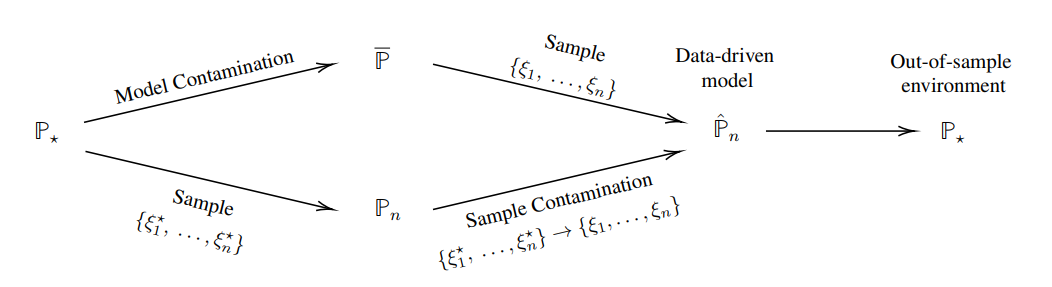
\includegraphics[width=0.85\textwidth]{images/img2.png}
    \caption{Decision Making Cycle in the Context of Robust Statistics}
    \label{fig2}
\end{figure}
In both cases, the learned model is constructed from corrupted information but is still intended to approximate the true distribution $\mathbb{P}^*$.

\section{Distributionally Robust Optimization (DRO)}
To address cases (i) and (ii), \textbf{distributionally robust optimization (DRO)}~\cite{rahimian2019distributionally} is a principled framework that seeks to minimize discrepancies between the \textit{in-sample expected loss} (under $\hat{\mathbb{P}}_n$) and the \textit{out-of-sample expected loss} (under $\tilde{\mathbb{P}}$). DRO explicitly accounts for distributional uncertainty to achieve more robust decision-making.

\subsection{Stochastic Optimization Setup}
\begin{itemize}[left=1em]
    \item Random vector: $\xi \in \Xi \subseteq \mathbb{R}^d$, let $\vec{z} = \xi$, distributed according to the true distribution $\mathbb{P}_\star$.  
    \item Model parameters: $\theta \in \Theta$ (assume finite-dimensional).  
    \item Loss function: $\ell(\vec{z}, \vec{\theta})$ measures the cost of using parameter $\vec{\theta}$ on data realization $\vec{z}$.  
\end{itemize}

\subsection{DRO Formulation}
ERM may lead to poor out-of-sample performance due to overfitting, distributional shift, or data contamination.  
To ensure robustness, DRO introduces an \textbf{uncertainty set} $\mathcal{B}(\hat{P}_n)$ around the empirical distribution, which captures possible deviations between in-sample and out-of-sample distributions.

The DRO problem is then formulated as:
\begin{equation}
    \min_{\vec{\theta} \in \Theta} \; \sup_{Q \in \mathcal{B}(\hat{\mathbb{P}}_n)} 
    \mathbb{E}_{Q} \big[ \ell(\vec{z}, \vec{\theta}) \big] = \hat{L}_r(\vec{z}, \vec{\theta}),
\end{equation}

where the inner $\sup$ considers the worst-case expected loss under all distributions $Q$ in the 

uncertainty set $\mathcal{B}(\hat{\mathbb{P}}_n)$.
\newpage 
\section{Distributional Uncertainty Sets}
\textbf{KEY QUESTION:} How do we measure distributional uncertainty?
\\
A key step in distributionally robust optimization (DRO) is the specification of the \textbf{distributional uncertainty set} $\mathcal{B}$. Different choices of $\mathcal{B}$ lead to different formulations of the DRO problem.

\subsection{Moment-Based Uncertainty Sets}
One of the earliest approaches~\cite{delage2010distributionally} models uncertainty using \textbf{moment constraints}.  
The general DRO problem is
\[
    \min_{\theta \in \Theta} \; \sup_{\mathbb{Q} \in \mathcal{B}} \, \mathbb{E}_\mathbb{Q}[\ell(\theta, z)],
\]
where the uncertainty set $\mathcal{B}$ is defined via constraints on the mean and covariance.

\paragraph{Construction of $\mathcal{B}$:}
Let $\hat{\mu}$ and $\hat{\Sigma}$ denote the empirical mean and covariance estimated from $\hat{\mathbb{P}}_n$.  
Given non-negative constants $\delta_1, \delta_2$, define
\[
    \mathcal{B} = \Bigg\{ \mathbb{Q} \;:\;
    \big(\mathbb{E}_\mathbb{Q}[z] - \hat{\mu}\big)^\top \hat{\Sigma}^{-1}\big(\mathbb{E}_\mathbb{Q}[z] - \hat{\mu}\big) \leq \delta_1, \;
    \mathbb{E}_\mathbb{Q}\!\left[(z - \hat{\mu})^\top(z - \hat{\mu}) \right] \preceq \delta_2 \hat{\Sigma}
    \Bigg\}.
\]
Note that the first condition is basically bounding the square of \textbf{Mahalanobis distance} to a constant.

\paragraph{Advantages:}
This formulation often admits a \textbf{semi-definite programming} (SDP) representation, making it computationally attractive.  

\paragraph{Limitations:}
From a statistical standpoint, $\mathcal{B}$ may contain distributions far from the empirical distribution $\hat{\mathbb{P}}_n$, even for small $\delta_1, \delta_2$. 
As $n \to \infty$, $\hat{\mathbb{P}}_n \overset{w.p. 1}{\rightarrow} \mathbb{P}_\star$ under i.i.d.\ assumptions, but the set $\mathcal{B}$ may still include distributions that may be far from $\mathbb{P_\star}$ (overly conservative). 
This conservatism may hurt performance, except in cases where the optimal solution only depends on first and second moments.  

\subsection{Metric-Based Uncertainty Sets}
A more modern and widely adopted approach defines the uncertainty set via a \textbf{probability metric/discrepancy} between distributions.  
Specifically, given a discrepancy measure $D(\cdot, \cdot)$ on the space of probability measures $\mathcal{P}(\Xi)$, define
\[
    \mathcal{B}_\delta(\hat{\mathbb{P}}_n) = \big\{ \mathbb{Q} \;:\; D(\mathbb{Q}, \hat{\mathbb{P}}_n) \leq \delta \big\}.
\]

Here, $\delta \geq 0$ defines the radius of a \textbf{ball} around $\hat{\mathbb{P}}_n$ with respect to the chosen discrepancy measure $D$.  

\paragraph{Advantages:}
Such sets capture distributions \textit{close} to the empirical distribution $\hat{\mathbb{P}}_n$.

\section{Distances between distributions}
\subsection{$\phi$-Divergence}
\subsubsection*{Absolute continuity}
A measure Q is said to be absolutely continuous w.r.t.\ measure P if for every $A \in \mathcal{F}$,
\begin{align*}
    P(A) = 0 \, \Rightarrow \, Q(A) = 0\\
    \text{OR}\\
    Q(A) > 0 \, \Rightarrow \, P(A) > 0
\end{align*}
Thus, $Q \ll P$.

\subsubsection*{Continuous R.V.s}
Let $\mathbb{P}_X (A) = \mathbb{P}(X \in A)$ which forms a probability space with $(\Omega, \mathcal{F}) \text{ where } \Omega = \mathbb{R}$, $X:\Omega \to \mathbb{R}$ and $\mathcal{F}$ is Borel $\sigma$-field.  
If $\mathbb{P}_X(A)$ is absolutely continuous w.r.t.\ the Lebesgue measure $\lambda$.
Then, by \textbf{Radon-Nikodym theorem}, there exists a $\mathcal{F}$-measurable function $p_X : X \to \left[0, \infty \right)$, such that for any $A \in \mathcal{F}$,
\[
    \mathbb{P}_X(A) = \int_{X^{-1}(A)} \, dP = \int_{A} \, p_X \, d\lambda.
\]
The function $p_X$ satisfying the above equality is commonly written as $\frac{d\mathbb{P}_X}{d\lambda}$ and is called \textbf{Radon-Nikodym deriavtive}.\\
In Probability Theory, this term is known as probability density function of a random variable.
Usually, $p_X = p(X) \text{ and } A = \left[a, b\right] \Rightarrow \mathbb{P}_X(\left[a, b\right]) = \int_{a}^{b} p(x) \, dx$.

\paragraph{Definition:} Assume $\phi : \mathbb{R}_{+} \to \left(-\infty, +\infty\right]$ is a convex function with $\phi(0) = \lim_{t \to 0^+} \phi(t),$ then the $\phi$-divergence between $\mathbb{Q}$ and $\hat{\mathbb{P}}_n$ is
\[
D_{\phi}(\mathbb{Q}, \hat{\mathbb{P}}_{n}) = 
    \begin{cases}
        \displaystyle \int_{\Xi} \phi \left(\frac{d\mathbb{Q}}{d\hat{\mathbb{P}}_{n}} \right) d\hat{\mathbb{P}}_{n}(z), & \quad \mathbb{Q} \ll \hat{\mathbb{P}}_{n}, \\
        +\infty, & \quad \text{otherwise}.
    \end{cases}
\]
Where, $\tfrac{d\mathbb{Q}}{d\hat{\mathbb{P}}_{n}}$ = likelihood ratio (Radon–Nikodym derivative) and $\mathbb{Q}$ is absolutely continuous w.r.t.\ $\hat{\mathbb{P}}_n$.\\
The intuition using this is that the adversary can re-weight the relative importance ($w_i = a_i$) of each
sample with a budget constraint ($\delta$). So, the adversary systematically explores how re-weighting can potentially
impact the performance of an estimator as measured by a given expected loss~\cite{duchi2021learning}. The bigger the reweighting, the larger the divergence.

\subsubsection*{Commonly used $\phi$-divergences}
Examples:
\begin{enumerate}
    \item KL divergence: $\phi(t) = t \log t$
    \item Reverse KL divergence: $\phi(t) = -\log t$
    \item Total Variation distance: $\varphi(t) = \tfrac{1}{2} |t - 1|$
    \item Jensen-Shannon divergence: $\varphi(t) = \tfrac{1}{2} \big( t \log t - (t+1)\log (\tfrac{t+1}{2}) \big)$
\end{enumerate}

\subsubsection*{KL Divergence:}
\textbf{Intuition:} 
\[
H(Q, P) - H(Q) 
= \sum_x Q(x) \log \frac{1}{P(x)} - \sum_x Q(x)\log \frac{1}{Q(x)}
\]
\[
\implies D_{\mathrm{KL}}(Q \| P) = \sum_x Q(x) \log \frac{Q(x)}{P(x)} 
\]

Thus, this implies Excess entropy from incorrect distribution.

\subsubsection*{Total Variation Distance}
\[
\mathrm{TV}(Q,P) = \int_{z} \frac{1}{2} \left| \frac{Q(x)}{P(x)} - 1 \right| P(x)\, dx 
= \frac{1}{2} \int_{z} |Q(x) - P(x)| dx 
= \sup_{A \in \mathcal{F}} |Q(A) - P(A)|
\]

\subsubsection*{Jensen-Shannon Divergence}
\[
\mathrm{JS}(Q,P) = \tfrac{1}{2} D_{\mathrm{KL}}\!\left(Q \Big\| \tfrac{Q+P}{2}\right) 
+ \tfrac{1}{2} D_{\mathrm{KL}}\!\left(P \Big\| \tfrac{Q+P}{2}\right)
\]

\paragraph{Notes}
\begin{enumerate}
    \item $D_{\mathrm{KL}}$ is not a metric (not symmetric, does not satisfies triangle inequality).
    \item Square root of $\mathrm{JS}$ is a metric.
    \item In $\phi$-divergence, $\mathbb{Q}$ is only supported where $\hat{\mathbb{P}}_n$ is supported.
\end{enumerate}

\subsubsection*{Properties of $\phi$-divergence}
\begin{enumerate}
\item Non-negativity:
    For any two probability distributions $Q$ and $P$,
    \[
        D_\phi(Q, P) \geq 0.
    \]
    \begin{proof}
    From the definition,
    \[
        D_\phi(Q, P) = \int_\Xi \phi\!\left(\frac{dQ}{dP}\right) dP,
    \]
    where $\phi : \mathbb{R}_+ \to (-\infty, +\infty]$ is convex with $\phi(1)=0$.\\
    By Jensen's inequality,
    \[
        \int_\Xi \phi\!\left(\frac{dQ}{dP}\right) dP \;\; \geq \;\; 
        \phi\!\left( \int_\Xi \frac{dQ}{dP} dP \right).
    \]
    Since $\int_\Xi \frac{dQ}{dP} dP = \int_\Xi dQ = 1$, the RHS equals $\phi(1)=0$.  
    Thus, $D_\phi(Q, P) \geq 0$.
    \end{proof}

\item Identity of indiscernibles:
    \[
        D_\phi(Q, P) = 0 \quad \iff \quad Q \overset{a.s.}= P \quad (\text{up to measure 0 set}).
    \]
    \begin{proof}
    If $Q = P$, then $\tfrac{dQ}{dP}=1$ everywhere and hence
    \[
        D_\phi(Q,P) = \int_\Xi \phi(1) dP = 0.
    \]
    Conversely, if $D_\phi(Q,P)=0$, then by strict convexity of $\phi$ (minimum at $t=1$), we must have
    \[
        \frac{dQ}{dP} = 1 \quad \text{$P$-almost surely}.
    \]
    This implies $Q=P$.
    \end{proof}
\end{enumerate}



% Optional, if you want to make a comment about vulnerability of any result or so on.
%\begin{danger}
%This is the danger environment.
%\end{danger}

\appendix
\chapter{Lebesgue integral with Dirac Measure}\label{adx1}
Let $(X,\mathcal{F})$ be a measurable space and fix $x \in X$.  
The Dirac measure at $x$, denoted $\delta_x$, is defined by
\[
\delta_x(A) =
\begin{cases}
1, & x \in A, \\
0, & x \notin A,
\end{cases}
\quad \forall A \in \mathcal{F}.
\]
We want to show that for any measurable function 
$f : X \to [-\infty,\infty]$,
\[
\int_{x} f(y) \, d\delta_x(y) = f(x),
\]
with the usual convention that the integral may take values $\pm \infty$ if $f$ is not integrable.  
When $f$ is integrable (i.e. $\int |f| \, d\delta_x < \infty$), the value is a finite real number equal to $f(x)$.
\section*{Proof}
\subsection*{Step 1: Indicator functions}

Let $A \in \mathcal{F}$. Then, by definition of the Lebesgue integral for indicator functions,
\[
\int_{x} \mathbf{1}_A(y) \, d\delta_x(y) = \delta_x(A) =
\begin{cases}
1, & x \in A, \\
0, & x \notin A.
\end{cases}
\]
But note that $\mathbf{1}_A(x)$ equals the same right-hand side. Hence
\[
\int_{x} \mathbf{1}_A \, d\delta_x = \mathbf{1}_A(x).
\]

\subsection*{Step 2: Simple functions}

Let $s = \sum_{k=1}^n a_k \mathbf{1}_{A_k}$ be a (nonnegative) simple function with $a_k \geq 0$ and $A_k \in \mathcal{F}$.  
Using linearity of the integral and Step 1,
\[
\int s \, d\delta_x = \sum_{k=1}^n a_k \int \mathbf{1}_{A_k} \, d\delta_x
= \sum_{k=1}^n a_k \, \mathbf{1}_{A_k}(x) = s(x).
\]

\subsection*{Step 3: Nonnegative measurable functions}

Let $f \geq 0$ be measurable. By construction of the Lebesgue integral, there exists an increasing sequence of simple functions $(s_n)$ with $0 \leq s_n \uparrow f$ pointwise.  
By the Monotone Convergence Theorem,
\[
\int f \, d\delta_x = \lim_{n \to \infty} \int s_n \, d\delta_x
= \lim_{n \to \infty} s_n(x) = f(x).
\]

\subsection*{Step 4: General measurable functions}

For a general measurable function $f$, write
\[
f = f^+ - f^-, \quad \text{where } f^+ = \max\{f,0\}, \; f^- = \max\{-f,0\}.
\]
If at least one of $\int f^\pm \, d\delta_x$ is $+\infty$, Step 3 implies
\[
\int f \, d\delta_x = f(x)
\]
in the extended sense.  
If $f$ is integrable (i.e. $\int |f| \, d\delta_x < \infty$), then applying Step 3 to $f^\pm$ and subtracting gives
\[
\int_{x} f \, d\delta_x = \int f^+ \, d\delta_x - \int f^- \, d\delta_x
= f^+(x) - f^-(x) = f(x).
\]

\bibliographystyle{plain}
\bibliography{refs}

\end{document}